% Options for packages loaded elsewhere
\PassOptionsToPackage{unicode}{hyperref}
\PassOptionsToPackage{hyphens}{url}
%
\documentclass[
  11pt,
]{article}
\usepackage{lmodern}
\usepackage{amssymb,amsmath}
\usepackage{ifxetex,ifluatex}
\ifnum 0\ifxetex 1\fi\ifluatex 1\fi=0 % if pdftex
  \usepackage[T1]{fontenc}
  \usepackage[utf8]{inputenc}
  \usepackage{textcomp} % provide euro and other symbols
\else % if luatex or xetex
  \usepackage{unicode-math}
  \defaultfontfeatures{Scale=MatchLowercase}
  \defaultfontfeatures[\rmfamily]{Ligatures=TeX,Scale=1}
\fi
% Use upquote if available, for straight quotes in verbatim environments
\IfFileExists{upquote.sty}{\usepackage{upquote}}{}
\IfFileExists{microtype.sty}{% use microtype if available
  \usepackage[]{microtype}
  \UseMicrotypeSet[protrusion]{basicmath} % disable protrusion for tt fonts
}{}
\makeatletter
\@ifundefined{KOMAClassName}{% if non-KOMA class
  \IfFileExists{parskip.sty}{%
    \usepackage{parskip}
  }{% else
    \setlength{\parindent}{0pt}
    \setlength{\parskip}{6pt plus 2pt minus 1pt}}
}{% if KOMA class
  \KOMAoptions{parskip=half}}
\makeatother
\usepackage{xcolor}
\IfFileExists{xurl.sty}{\usepackage{xurl}}{} % add URL line breaks if available
\IfFileExists{bookmark.sty}{\usepackage{bookmark}}{\usepackage{hyperref}}
\hypersetup{
  pdftitle={Research Project - Software Engineering 2},
  pdfauthor={Marco Molè},
  hidelinks,
  pdfcreator={LaTeX via pandoc}}
\urlstyle{same} % disable monospaced font for URLs
\usepackage{listings}
\newcommand{\passthrough}[1]{#1}
\lstset{defaultdialect=[5.3]Lua}
\lstset{defaultdialect=[x86masm]Assembler}
\usepackage{color}
\usepackage{fancyvrb}
\newcommand{\VerbBar}{|}
\newcommand{\VERB}{\Verb[commandchars=\\\{\}]}
\DefineVerbatimEnvironment{Highlighting}{Verbatim}{commandchars=\\\{\}}
% Add ',fontsize=\small' for more characters per line
\newenvironment{Shaded}{}{}
\newcommand{\AlertTok}[1]{\textcolor[rgb]{1.00,0.00,0.00}{\textbf{#1}}}
\newcommand{\AnnotationTok}[1]{\textcolor[rgb]{0.38,0.63,0.69}{\textbf{\textit{#1}}}}
\newcommand{\AttributeTok}[1]{\textcolor[rgb]{0.49,0.56,0.16}{#1}}
\newcommand{\BaseNTok}[1]{\textcolor[rgb]{0.25,0.63,0.44}{#1}}
\newcommand{\BuiltInTok}[1]{#1}
\newcommand{\CharTok}[1]{\textcolor[rgb]{0.25,0.44,0.63}{#1}}
\newcommand{\CommentTok}[1]{\textcolor[rgb]{0.38,0.63,0.69}{\textit{#1}}}
\newcommand{\CommentVarTok}[1]{\textcolor[rgb]{0.38,0.63,0.69}{\textbf{\textit{#1}}}}
\newcommand{\ConstantTok}[1]{\textcolor[rgb]{0.53,0.00,0.00}{#1}}
\newcommand{\ControlFlowTok}[1]{\textcolor[rgb]{0.00,0.44,0.13}{\textbf{#1}}}
\newcommand{\DataTypeTok}[1]{\textcolor[rgb]{0.56,0.13,0.00}{#1}}
\newcommand{\DecValTok}[1]{\textcolor[rgb]{0.25,0.63,0.44}{#1}}
\newcommand{\DocumentationTok}[1]{\textcolor[rgb]{0.73,0.13,0.13}{\textit{#1}}}
\newcommand{\ErrorTok}[1]{\textcolor[rgb]{1.00,0.00,0.00}{\textbf{#1}}}
\newcommand{\ExtensionTok}[1]{#1}
\newcommand{\FloatTok}[1]{\textcolor[rgb]{0.25,0.63,0.44}{#1}}
\newcommand{\FunctionTok}[1]{\textcolor[rgb]{0.02,0.16,0.49}{#1}}
\newcommand{\ImportTok}[1]{#1}
\newcommand{\InformationTok}[1]{\textcolor[rgb]{0.38,0.63,0.69}{\textbf{\textit{#1}}}}
\newcommand{\KeywordTok}[1]{\textcolor[rgb]{0.00,0.44,0.13}{\textbf{#1}}}
\newcommand{\NormalTok}[1]{#1}
\newcommand{\OperatorTok}[1]{\textcolor[rgb]{0.40,0.40,0.40}{#1}}
\newcommand{\OtherTok}[1]{\textcolor[rgb]{0.00,0.44,0.13}{#1}}
\newcommand{\PreprocessorTok}[1]{\textcolor[rgb]{0.74,0.48,0.00}{#1}}
\newcommand{\RegionMarkerTok}[1]{#1}
\newcommand{\SpecialCharTok}[1]{\textcolor[rgb]{0.25,0.44,0.63}{#1}}
\newcommand{\SpecialStringTok}[1]{\textcolor[rgb]{0.73,0.40,0.53}{#1}}
\newcommand{\StringTok}[1]{\textcolor[rgb]{0.25,0.44,0.63}{#1}}
\newcommand{\VariableTok}[1]{\textcolor[rgb]{0.10,0.09,0.49}{#1}}
\newcommand{\VerbatimStringTok}[1]{\textcolor[rgb]{0.25,0.44,0.63}{#1}}
\newcommand{\WarningTok}[1]{\textcolor[rgb]{0.38,0.63,0.69}{\textbf{\textit{#1}}}}
\usepackage{longtable,booktabs}
% Correct order of tables after \paragraph or \subparagraph
\usepackage{etoolbox}
\makeatletter
\patchcmd\longtable{\par}{\if@noskipsec\mbox{}\fi\par}{}{}
\makeatother
% Allow footnotes in longtable head/foot
\IfFileExists{footnotehyper.sty}{\usepackage{footnotehyper}}{\usepackage{footnote}}
\makesavenoteenv{longtable}
\usepackage{graphicx}
\makeatletter
\def\maxwidth{\ifdim\Gin@nat@width>\linewidth\linewidth\else\Gin@nat@width\fi}
\def\maxheight{\ifdim\Gin@nat@height>\textheight\textheight\else\Gin@nat@height\fi}
\makeatother
% Scale images if necessary, so that they will not overflow the page
% margins by default, and it is still possible to overwrite the defaults
% using explicit options in \includegraphics[width, height, ...]{}
\setkeys{Gin}{width=\maxwidth,height=\maxheight,keepaspectratio}
% Set default figure placement to htbp
\makeatletter
\def\fps@figure{htbp}
\makeatother
% Make links footnotes instead of hotlinks:
\DeclareRobustCommand{\href}[2]{#2\footnote{\url{#1}}}
\setlength{\emergencystretch}{3em} % prevent overfull lines
\providecommand{\tightlist}{%
  \setlength{\itemsep}{0pt}\setlength{\parskip}{0pt}}
\setcounter{secnumdepth}{5}

\title{Research Project - Software Engineering 2}
\author{Marco Molè}
\date{AA 2022/2023}

\begin{document}
\maketitle

{
\setcounter{tocdepth}{3}
\tableofcontents
}
\hypertarget{introduction}{%
\section{Introduction}\label{introduction}}

Kubernetes, also known as K8s, is an open-source container orchestration
platform designed to automate the deployment, scaling, and management of
containerized applications. Originally developed by Google and later
donated to the Cloud Native Computing Foundation, Kubernetes is now
widely used in cloud computing environments to manage the deployment of
containerized applications across a cluster of nodes.

At its core, Kubernetes operates by organizing containers into logical
units called pods, which are then deployed and managed as a single
entity. These pods are designed to be highly portable and can be
deployed across a range of cloud and on-premises environments, enabling
organizations to build and deploy applications in a way that is both
scalable and cost-effective.

One of the key benefits of Kubernetes is its ability to automate many of
the tasks associated with managing containerized applications, including
load balancing, scaling, and failover. This automation not only helps to
reduce the operational overhead of managing large-scale container
deployments but also ensures that applications are always available and
running smoothly.

Overall, Kubernetes represents a significant advancement in the field of
container orchestration, providing developers and operations teams with
a powerful tool for managing containerized applications at scale. As
such, it has become an essential technology for organizations looking to
leverage the benefits of containerization and cloud computing to build
more agile, scalable, and resilient applications.

The Kubernetes configuration language is expressed in YAML or JSON
format, and it consists of a set of declarative statements that describe
the desired state of the Kubernetes resources. These statements include
specifications for the containers that run within the resources, as well
as other settings such as environment variables, ports, and volumes.

In this report I'll explore how the declarative language is used to
define the main kubernetes objects. Then I'll propose a mechanism for
simplifying the process of writing correct configurations of Pods.

\hypertarget{how-kubernetes-works}{%
\subsection{How kubernetes works}\label{how-kubernetes-works}}

At its core, Kubernetes is built around the concept of a cluster, which
is a group of machines (called nodes) that work together to run
containerized applications. The Kubernetes control plane, which is
responsible for managing the cluster, consists of several components
that work together to provide a robust and scalable platform for
deploying and managing containerized applications.

One of the key concepts in Kubernetes is the pod, which is the smallest
deployable unit in the system. A pod is a logical host for one or more
containers, and it provides a shared environment for those containers to
run in. Each pod has a unique IP address and hostname, which makes it
easy to communicate with other pods in the same cluster.

The Kubernetes control plane consists of several components, including
the API server, etcd, the scheduler, and the controller manager. The API
server provides a RESTful API that users can use to interact with the
Kubernetes cluster. Etcd is a distributed key-value store that stores
the configuration data for the cluster, such as the desired state of the
system. The scheduler is responsible for assigning pods to nodes in the
cluster based on various criteria, such as resource availability and
affinity. Finally, the controller manager is responsible for ensuring
that the current state of the cluster matches the desired state.

Kubernetes also provides several key features that make it easy to
manage containerized applications, such as service discovery, load
balancing, and auto-scaling. Service discovery allows applications to
easily find and communicate with other services in the same cluster.
Load balancing ensures that traffic is distributed evenly across all
instances of a service, while auto-scaling makes it easy to
automatically scale the number of instances up or down based on demand.

\hypertarget{main-components}{%
\section{Main components}\label{main-components}}

In this section I'll provide a more detailed explanation of the most
important components.

\hypertarget{pods}{%
\subsection{Pods}\label{pods}}

In Kubernetes, a pod is the smallest deployable unit that can be
created, scheduled, and managed. Pods can contain one or more
containers, which share the same network namespace and can communicate
with each other using inter-process communication (IPC). The declarative
language of Kubernetes is used to define pods in a Kubernetes manifest
file, which is a YAML or JSON file that describes the desired state of
the pod.

To define a pod using Kubernetes' declarative language, the manifest
file must include the following information:

\begin{enumerate}
\def\labelenumi{\arabic{enumi}.}
\item
  metadata: This includes information such as the name and labels of the
  pod.
\item
  spec: This includes information about the desired state of the pod,
  such as the containers it should contain, the image(s) to use, and the
  commands to run. In this section, you can also specify the ports to
  expose, any environment variables to set, and any volumes to mount.
\end{enumerate}

For example, the following YAML manifest file defines a pod with one
container:

\begin{Shaded}
\begin{Highlighting}[]
\FunctionTok{apiVersion}\KeywordTok{:}\AttributeTok{ v1}
\FunctionTok{kind}\KeywordTok{:}\AttributeTok{ Pod}
\FunctionTok{metadata}\KeywordTok{:}
\AttributeTok{  }\FunctionTok{name}\KeywordTok{:}\AttributeTok{ my{-}pod}
\AttributeTok{  }\FunctionTok{labels}\KeywordTok{:}
\AttributeTok{    }\FunctionTok{app}\KeywordTok{:}\AttributeTok{ my{-}app}
\FunctionTok{spec}\KeywordTok{:}
\AttributeTok{  }\FunctionTok{containers}\KeywordTok{:}
\AttributeTok{  }\KeywordTok{{-}}\AttributeTok{ }\FunctionTok{name}\KeywordTok{:}\AttributeTok{ my{-}container}
\AttributeTok{    }\FunctionTok{image}\KeywordTok{:}\AttributeTok{ nginx}
\AttributeTok{    }\FunctionTok{ports}\KeywordTok{:}
\AttributeTok{    }\KeywordTok{{-}}\AttributeTok{ }\FunctionTok{containerPort}\KeywordTok{:}\AttributeTok{ }\DecValTok{80}
\end{Highlighting}
\end{Shaded}

In this example, the manifest file specifies that the pod should be
named ``my-pod'' and labeled with ``app: my-app''. It also specifies
that the pod should contain one container named ``my-container'' that
runs the Nginx image and exposes port 80.

Once the manifest file has been created, it can be applied to the
Kubernetes cluster using the \emph{kubectl apply} command. Kubernetes
will then compare the desired state specified in the manifest file with
the actual state of the cluster and make any necessary changes to ensure
that the desired state is achieved.

\hypertarget{deployments}{%
\subsection{Deployments}\label{deployments}}

A deployment is an object that defines the desired state of a set of
replicated pods. Deployments are a higher-level abstraction that enables
declarative updates to the desired state of the pod set, allowing for
easier management of the underlying resources.

A Kubernetes deployment is responsible for creating and managing a
ReplicaSet, which is a Kubernetes object that ensures a specified number
of identical replicas of a pod are running at any given time.
Deployments provide a way to manage the scaling and rolling updates of
pods, by automating the creation and deletion of replica sets as
necessary. The deployment object also provides rollback and pause/resume
functionality, allowing for more fine-grained control over the lifecycle
of the pod set.

When creating a Kubernetes deployment, a user specifies the desired
number of replicas, the container images and configurations, and the
update strategy. The deployment controller then uses this information to
ensure that the desired state of the pod set is achieved and maintained.
If the actual state of the pod set deviates from the desired state, the
deployment controller automatically performs rolling updates, scaling,
or deletion of pods as necessary.

Deployments are a critical component of the Kubernetes platform, as they
enable users to manage containerized applications at scale with ease. By
abstracting away the complexity of managing individual pods, Kubernetes
deployments provide a higher-level interface that is more intuitive for
users and reduces the potential for human error. With Kubernetes
deployments, users can confidently manage their applications in a highly
available and fault-tolerant manner.

To define a deployment using Kubernetes' declarative language, the
manifest file must include the following information:

\begin{enumerate}
\def\labelenumi{\arabic{enumi}.}
\item
  metadata: This includes information such as the name and labels of the
  deployment.
\item
  spec: This includes information about the desired state of the
  deployment, such as the number of replicas, the selector that
  identifies the pods managed by the deployment, and the configuration
  of the containers. For example, the following YAML manifest file
  defines a deployment with 3 replicas:
\end{enumerate}

\begin{Shaded}
\begin{Highlighting}[]
\FunctionTok{apiVersion}\KeywordTok{:}\AttributeTok{ apps/v1}
\FunctionTok{kind}\KeywordTok{:}\AttributeTok{ Deployment}
\FunctionTok{metadata}\KeywordTok{:}
\AttributeTok{  }\FunctionTok{name}\KeywordTok{:}\AttributeTok{ my{-}deployment}
\FunctionTok{spec}\KeywordTok{:}
\AttributeTok{  }\FunctionTok{replicas}\KeywordTok{:}\AttributeTok{ }\DecValTok{3}
\AttributeTok{  }\FunctionTok{selector}\KeywordTok{:}
\AttributeTok{    }\FunctionTok{matchLabels}\KeywordTok{:}
\AttributeTok{      }\FunctionTok{app}\KeywordTok{:}\AttributeTok{ my{-}app}
\AttributeTok{  }\FunctionTok{template}\KeywordTok{:}
\AttributeTok{    }\FunctionTok{metadata}\KeywordTok{:}
\AttributeTok{      }\FunctionTok{labels}\KeywordTok{:}
\AttributeTok{        }\FunctionTok{app}\KeywordTok{:}\AttributeTok{ my{-}app}
\AttributeTok{    }\FunctionTok{spec}\KeywordTok{:}
\AttributeTok{      }\FunctionTok{containers}\KeywordTok{:}
\AttributeTok{      }\KeywordTok{{-}}\AttributeTok{ }\FunctionTok{name}\KeywordTok{:}\AttributeTok{ my{-}container}
\AttributeTok{        }\FunctionTok{image}\KeywordTok{:}\AttributeTok{ nginx}
\AttributeTok{        }\FunctionTok{ports}\KeywordTok{:}
\AttributeTok{        }\KeywordTok{{-}}\AttributeTok{ }\FunctionTok{containerPort}\KeywordTok{:}\AttributeTok{ }\DecValTok{80}
\end{Highlighting}
\end{Shaded}

In this example, the manifest file specifies that the deployment should
be named ``my-deployment'' and should include three replicas. It also
specifies that the deployment should manage pods labeled with ``app:
my-app'' and should create pods with one container running the Nginx
image and exposing port 80.

\hypertarget{services}{%
\subsection{Services}\label{services}}

A Service is an abstraction that enables a stable IP address and DNS
name to be assigned to a set of Pods. In essence, it serves as a
mechanism for defining a logical grouping of Pods and providing a single
point of access to them, regardless of the specific Pod that a client
may be communicating with at any given time. Services are typically used
to enable load balancing and horizontal scaling of application
components running within a Kubernetes cluster.

A Service is defined through a declarative YAML configuration file,
which specifies the selector label that matches the Pods to be included
in the Service, as well as the port(s) that the Service should expose.
When a Service is created, Kubernetes automatically assigns it a
cluster-unique IP address and creates an associated DNS entry. Requests
sent to the Service's IP address and port are then automatically routed
to one of the available Pods that match the Service's selector, based on
a simple round-robin algorithm. This allows clients to access the
application components running within a Kubernetes cluster in a
consistent and scalable manner, without needing to know the specific IP
addresses or hostnames of individual Pods.

Service can be configured in several ways depending on the requirements
of the application or workload. Some of the common configurations
include:

\begin{enumerate}
\def\labelenumi{\arabic{enumi}.}
\item
  ClusterIP: This is the default configuration for a Service and
  provides a stable IP address and DNS name within the cluster. The
  Service is only accessible from within the cluster and is not exposed
  to the external network.
\item
  NodePort: This configuration exposes the Service on a static port on
  each node in the cluster. This allows the Service to be accessed from
  outside the cluster using the node's IP address and the static port
  number.
\item
  LoadBalancer: This configuration creates a load balancer in a cloud
  provider's network, which distributes incoming traffic to the Service
  across multiple nodes. This is typically used when external traffic
  needs to be distributed across multiple nodes or when a high degree of
  availability is required.
\item
  ExternalName: This configuration provides a way to create a Service
  that simply maps to an external DNS name. This is useful when an
  application needs to access an external resource, such as a database
  or web service, using a stable DNS name.
\end{enumerate}

In addition to these basic configurations, Services can also be combined
with other Kubernetes features such as selectors, labels, and endpoints
to provide more advanced functionality. For example, Services can be
used in conjunction with Ingress controllers to provide an HTTP(S) load
balancer that routes traffic based on the URL path or hostname of
incoming requests.

\hypertarget{volumes}{%
\subsection{Volumes}\label{volumes}}

A volume is a directory accessible to containers in a Pod. A volume can
be used to store data that needs to be shared between containers, or to
persist data beyond the lifetime of a container. Volumes in Kubernetes
are defined using a declarative configuration file in YAML format.

There are several types of volumes that can be used in Kubernetes,
including hostPath volumes, emptyDir volumes, configMap volumes, secret
volumes, and persistent volumes. HostPath volumes mount a directory from
the host into the container, while emptyDir volumes are created when a
Pod is scheduled on a node and deleted when the Pod is terminated.
ConfigMap volumes and secret volumes provide a way to inject
configuration data or sensitive information into a container,
respectively. Persistent volumes are used to store data beyond the
lifetime of a Pod, and can be dynamically provisioned or statically
created by an administrator.

To define a volume in Kubernetes, the YAML configuration file would
include a volumes section with the desired volume type and configuration
options. For example, to define a hostPath volume that mounts the /data
directory from the host into a container, the YAML file would look like:

\begin{Shaded}
\begin{Highlighting}[]

\FunctionTok{apiVersion}\KeywordTok{:}\AttributeTok{ v1}
\FunctionTok{kind}\KeywordTok{:}\AttributeTok{ Pod}
\FunctionTok{metadata}\KeywordTok{:}
\AttributeTok{  }\FunctionTok{name}\KeywordTok{:}\AttributeTok{ my{-}pod}
\FunctionTok{spec}\KeywordTok{:}
\AttributeTok{  }\FunctionTok{containers}\KeywordTok{:}
\AttributeTok{  }\KeywordTok{{-}}\AttributeTok{ }\FunctionTok{name}\KeywordTok{:}\AttributeTok{ my{-}container}
\AttributeTok{    }\FunctionTok{image}\KeywordTok{:}\AttributeTok{ my{-}image}
\AttributeTok{    }\FunctionTok{volumeMounts}\KeywordTok{:}
\AttributeTok{    }\KeywordTok{{-}}\AttributeTok{ }\FunctionTok{name}\KeywordTok{:}\AttributeTok{ my{-}volume}
\AttributeTok{      }\FunctionTok{mountPath}\KeywordTok{:}\AttributeTok{ /data}
\AttributeTok{  }\FunctionTok{volumes}\KeywordTok{:}
\AttributeTok{  }\KeywordTok{{-}}\AttributeTok{ }\FunctionTok{name}\KeywordTok{:}\AttributeTok{ my{-}volume}
\AttributeTok{    }\FunctionTok{hostPath}\KeywordTok{:}
\AttributeTok{      }\FunctionTok{path}\KeywordTok{:}\AttributeTok{ /data}
\end{Highlighting}
\end{Shaded}

This configuration file specifies that a hostPath volume named
\emph{my-volume} should be mounted at \emph{/data }inside the container.
The \emph{volumeMounts} field in the container specification specifies
which volume to mount, and where to mount it.

\hypertarget{my-contribution}{%
\section{My contribution}\label{my-contribution}}

\hypertarget{the-problem}{%
\subsection{The Problem}\label{the-problem}}

When writing the specification of a Pod one can specify the container
images to run and from which registry pull it from. Container registries
are software repositories that store and distribute container images. A
container registry is typically used by developers and DevOps teams to
store and manage container images, which can be easily shared across
different environments, such as development, staging, and production.
Container registries provide features like versioning, access control,
and image scanning to ensure that container images are secure, reliable,
and up-to-date.

Most often, images require configuration through the use of environment
variables. The documentation of these variables is generally found on
the registry itself, to be consulted by the developer when writing the
specification of the Pod.

Configuration errors could be caused by human error, either neglecting
to read the documentation, or by misinterpreting it, or by the lack of
documentation of the image itself. Misconfiguration could lead to the
application not working as expected, or not working at all. It also
could be a security risk, since a misconfiguration of security
parameters could lead to the use of default credentials, or to the use
of a non secure protocol.

An erroneous configuration of a container is hard to debug, since the
point of failure may not be immediately recognizable due to the highly
level of coupling of microservices architecture. There is also an
additional element of complexity due to the fact that the application is
running inside a virtualized environment, and the failure could be
caused by a misconfiguration of the container itself.

The manifestations of these errors are mainly two: the application does
not work as expected, or it does not work at all. The first case happens
when the misconfiguration is not critical, and the application is still
able to run, but with some functionalities not working as expected. For
example, the application could be running with some default
configuration that does not expose all the functionalities of the
application.

The second case happens when the misconfiguration is critical, and the
application is not able to run at all. For example, no credentials are
provided to the application, and the application is not able to connect
to the database.

In both cases, the developer has to debug the application to find the
cause of the error, and then fix it. This is a time consuming process,
since the developer has to find the cause of the error, and then fix it.

It could be also a potentially costly error, since most of K8s clusters
exist on a pay-per-use cloud environment.

There is no automatic mechanism that inform the developer if the
configuration they have written is correct, or at least if it satisfies
some minimum configuration requirements.

\hypertarget{a-possible-solution}{%
\subsection{A Possible Solution}\label{a-possible-solution}}

This mechanism could be included in the development environment, for
example as a LSP language server. The solution I propose is to provide a
mechanism that allows the developer to check if the configuration they
have written satisfies some minimum configuration requirements, defined
by the maintainer of the image. This minimum configuration schema is
stored in the registry, and is accessible by the developer's IDE when
writing the specification of the Pod. The developer can then check if
the configuration they have written satisfies the minimum configuration
requirements, and if not, the IDE will inform the developer of the
missing configuration options, and the type of the configuration
options.

The
\href{https://microsoft.github.io/language-server-protocol/}{Language
Server Protocol (LSP)} is a communication protocol that enables the
integration of programming language analyzers, such as code editors,
with language servers that provide language-specific features such as
code completion, error detection, and refactoring. The protocol
standardizes the exchange of information between the language server and
the client, allowing for interoperability between different code editors
and programming languages. This can help developers work more
efficiently by providing consistent, language-specific tools across
different editing environments.

\hypertarget{schema-of-the-configuration-options}{%
\subsubsection{Schema of the configuration
options}\label{schema-of-the-configuration-options}}

The schema of the configuration options is a JSON object that specifies
the configuration options of the image, and the type of each
configuration option. The schema should contain information about the
mandatory configuration options, and the facultative configuration
options. The schema should also contain information about the default
value of the facultative configuration options.

\newpage

The format of the schema could be generalized to this structure:

\begin{Shaded}
\begin{Highlighting}[]
\FunctionTok{\{}
  \DataTypeTok{"image"} \FunctionTok{:} \StringTok{"name of the image:version"}\FunctionTok{,}
  \DataTypeTok{"example\_of\_mandatory\_configuration\_option"} \FunctionTok{:} \FunctionTok{\{}
    \DataTypeTok{"mandatory"} \FunctionTok{:} \KeywordTok{true}\FunctionTok{,}
    \DataTypeTok{"type"}\FunctionTok{:}\StringTok{"type of the configuration option"}\FunctionTok{,}
  \FunctionTok{\},}
  \DataTypeTok{"example\_of\_facultative\_configuration\_option"} \FunctionTok{:} \FunctionTok{\{}
    \DataTypeTok{"mandatory"} \FunctionTok{:} \KeywordTok{false}\FunctionTok{,}
    \DataTypeTok{"type"}\FunctionTok{:}\StringTok{"type of the configuration option"}\FunctionTok{,}
    \DataTypeTok{"default"}\FunctionTok{:} \StringTok{"default value of the configuration option"}
  \FunctionTok{\},}
\FunctionTok{\}}
\end{Highlighting}
\end{Shaded}

The type of the configuration option could be one of the following:
string, number, path (ie a string that represents a path), boolean etc.
More types definition could be added if needed.

An interesting case is the case of the default value of a facultative
configuration option. The default value could be a string, or it could
be the value of another configuration option. In the latter case, the
value of the default value should be a string that represents the name
of the configuration option, preceded by the \emph{\$} symbol. The
\emph{\$} symbol is used to express that the default value is the value
of another configuration option.

This could be useful in the case of a configuration option that is
facultative, but that has a default value that depends on the value of
another configuration option. This is the case of the configuration
options of the postgres image, where the default value of the
POSTGRES\_DB configuration option is the value of the POSTGRES\_USER
configuration option.

\begin{Shaded}
\begin{Highlighting}[]
\FunctionTok{\{}
  \DataTypeTok{"image"}\FunctionTok{:} \StringTok{"postgres:latest"}\FunctionTok{,}
  \DataTypeTok{"POSTGRES\_PASSWORD"} \FunctionTok{:} \FunctionTok{\{}
    \DataTypeTok{"mandatory"} \FunctionTok{:} \KeywordTok{true}\FunctionTok{,}
    \DataTypeTok{"type"}\FunctionTok{:}\StringTok{"string"}
  \FunctionTok{\},}
  \DataTypeTok{"POSTGRES\_USER"} \FunctionTok{:} \FunctionTok{\{}
    \DataTypeTok{"mandatory"} \FunctionTok{:} \KeywordTok{false}\FunctionTok{,}
    \DataTypeTok{"type"}\FunctionTok{:}\StringTok{"string"}\FunctionTok{,}
    \DataTypeTok{"default"}\FunctionTok{:} \StringTok{"postgres"}
  \FunctionTok{\},}
  \DataTypeTok{"POSTGRES\_DB"} \FunctionTok{:} \FunctionTok{\{}
    \DataTypeTok{"mandatory"} \FunctionTok{:} \KeywordTok{false}\FunctionTok{,}
    \DataTypeTok{"type"}\FunctionTok{:}\StringTok{"string"}\FunctionTok{,}
    \DataTypeTok{"default"}\FunctionTok{:} \StringTok{"$POSTGRES\_USER"}
  \FunctionTok{\}}
\FunctionTok{\}}
\end{Highlighting}
\end{Shaded}

Another case is when the default value of a facultative configuration
option is a random and auto-generated value. In this case, the value of
the default value is written as ``!random''. An example of this is the
DOCKER\_INFLUXDB\_INIT\_ADMIN\_TOKEN variable, which can be found in the
example section.

\hypertarget{another-proposal-for-the-notion-of-type-in-this-context-using-regular-expressions}{%
\paragraph{Another proposal for the notion of type in this context using
regular
expressions}\label{another-proposal-for-the-notion-of-type-in-this-context-using-regular-expressions}}

An alternative to strictly defining the type of the configuration option
is to define a regular expression that the value of the configuration
option should satisfy. This could be useful in the case of a
configuration option that is a string, but that has to satisfy some
constraints. For example, the value of the configuration option could be
a string that represents a path, and the regular expression could be
used to check if the string is a valid path.

So, for example, instead of defining the type of the configuration
option as ``path'', the type of the configuration option could be
defined as a regular expression that represents a valid path, like:

\begin{longtable}[]{@{}ll@{}}
\caption{Some examples of types and their corresponding regular
expressions}\tabularnewline
\toprule
Type & regex\tabularnewline
\midrule
\endfirsthead
\toprule
Type & regex\tabularnewline
\midrule
\endhead
string & .*\tabularnewline
number & {[}0-9{]}+\tabularnewline
float & {[}0-9{]}+.{[}0-9{]}+\tabularnewline
path & \^{}/({[}A-z0-9/-\_{]}+)/\$\tabularnewline
boolean & true\textbar false\tabularnewline
domain &
\^{}({[}a-z0-9{]}+(-{[}a-z0-9{]}+)*.)+{[}a-z{]}\{2,\}\$\tabularnewline
ipv4 & \^{}({[}0-9{]}\{1,3\}.)\{3\}{[}0-9{]}\{1,3\}\$\tabularnewline
ipv6 &
\^{}({[}0-9a-f{]}\{1,4\}:)\{7\}({[}0-9a-f{]})\{1,4\}\$\tabularnewline
url &
{[}-a-zA-Z0-9@:\%\_+.\textasciitilde\#?\&//={]}\{2,256\}.{[}a-z{]}\{2,4\}\b(/{[}-a-zA-Z0-9@:\%\_+.\textasciitilde\#?\&//={]}*)?\tabularnewline
\bottomrule
\end{longtable}

This approach is more flexible than the previous one, since it allows to
define the type of the configuration option in a more precise way.
However, it is also more complex, since it requires the definition of a
regular expression for each type of configuration option. This could be
a problem in the case of complex types, like the url type. In this case,
the regular expression is very complex, and it is not easy to understand
what it does.

If the regex approach is used, the schema of the configuration options
could be generalized to this structure:

\begin{Shaded}
\begin{Highlighting}[]
\FunctionTok{\{}
  \DataTypeTok{"image"} \FunctionTok{:} \StringTok{"name of the image:version"}\FunctionTok{,}
  \DataTypeTok{"example\_of\_mandatory\_configuration\_option"} \FunctionTok{:} \FunctionTok{\{}
    \DataTypeTok{"mandatory"} \FunctionTok{:} \KeywordTok{true}\FunctionTok{,}
    \DataTypeTok{"regex"}\FunctionTok{:}\StringTok{"regular expression that the value of the configuration option should satisfy"}\FunctionTok{,}
  \FunctionTok{\},}
  \DataTypeTok{"example\_of\_facultative\_configuration\_option"} \FunctionTok{:} \FunctionTok{\{}
    \DataTypeTok{"mandatory"} \FunctionTok{:} \KeywordTok{false}\FunctionTok{,}
    \DataTypeTok{"regex"}\FunctionTok{:}\StringTok{"regular expression that the value of the configuration option should satisfy"}\FunctionTok{,}
    \DataTypeTok{"default"}\FunctionTok{:} \StringTok{"default value of the configuration option"}
  \FunctionTok{\},}
\FunctionTok{\}}
\end{Highlighting}
\end{Shaded}

\hypertarget{protocol-for-the-communication-between-the-ide-and-the-registry}{%
\subsubsection{Protocol for the communication between the IDE and the
registry}\label{protocol-for-the-communication-between-the-ide-and-the-registry}}

The registries should offer an HTTP endpoint that replies with the
configuration schema of the requested image, to be consumed by the IDE.

The flow of the interaction between the parties is shown in the
following sequence diagram.

\begin{figure}
\centering
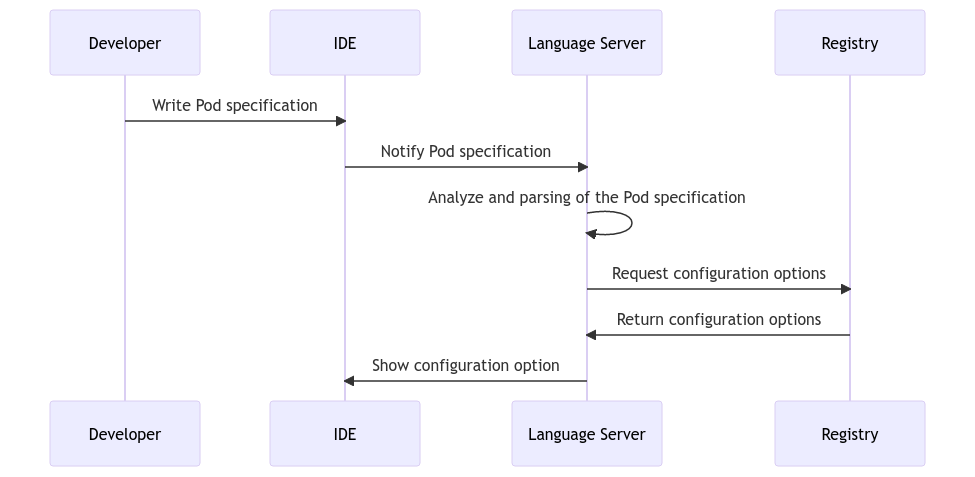
\includegraphics{./sweng2-rp-mole/diagrams/api.png}
\caption{Sequence Diagram of the interaction between the parties}
\end{figure}

The developer writes the specification of the Pod in a YAML file, and
the IDE sends a request to the registry to retrieve the configuration
options of the specified image.

This solution provides very little overhead on the registry, since the
registry only has to reply to the request of the IDE with the
configuration schema of the requested image. The registry does not have
to store any additional information, since the configuration schema is
stored in the registry as a JSON object.

This information is then checked against the PodSpec.containers.env
object, which is the object where all the environment variables of the
specific containers are specified. The results of this analysis are then
shown to the user as warnings or error marks in the IDE.

Recall how kubernetes objects are structured. The PodSpec.containers.env
object is a list of key-value pairs. The key is the name of the
environment variable, and the value is the value of the environment
variable. Environment variables must be defined as a string.

\begin{Shaded}
\begin{Highlighting}[]
\FunctionTok{apiVersion}\KeywordTok{:}\AttributeTok{ v1}
\FunctionTok{kind}\KeywordTok{:}\AttributeTok{ Pod}
\FunctionTok{metadata}\KeywordTok{:}
\AttributeTok{  }\FunctionTok{name}\KeywordTok{:}\AttributeTok{ nginx}
\FunctionTok{spec}\KeywordTok{:}\CommentTok{  \# PodSpec}
\AttributeTok{  }\FunctionTok{containers}\KeywordTok{:}\CommentTok{ \# PodSpec.containers}
\AttributeTok{  }\KeywordTok{{-}}\AttributeTok{ }\FunctionTok{name}\KeywordTok{:}\AttributeTok{ nginx}
\AttributeTok{    }\FunctionTok{image}\KeywordTok{:}\AttributeTok{ nginx}
\AttributeTok{    }\FunctionTok{env}\KeywordTok{:}\CommentTok{ \# PodSpec.containers.env}
\AttributeTok{    }\KeywordTok{{-}}\AttributeTok{ }\FunctionTok{name}\KeywordTok{:}\AttributeTok{ ENVIRONMENT }
\AttributeTok{      }\FunctionTok{value}\KeywordTok{:}\AttributeTok{ }\StringTok{"production"}
\AttributeTok{    }\KeywordTok{{-}}\AttributeTok{ }\FunctionTok{name}\KeywordTok{:}\AttributeTok{ LOG\_LEVEL}
\AttributeTok{      }\FunctionTok{value}\KeywordTok{:}\AttributeTok{ }\StringTok{"INFO"}
\end{Highlighting}
\end{Shaded}

\hypertarget{how-the-language-server-checks-the-configuration-options}{%
\paragraph{How the Language Server checks the configuration
options}\label{how-the-language-server-checks-the-configuration-options}}

The
\href{https://microsoft.github.io/language-server-protocol/specifications/lsp/3.17/specification/}{Language
Server Protocol specification} provides a set of methods that the IDE
can use to communicate with the Language Server. The methods that are
used in this context are:

\begin{itemize}
\item
  initialize: The initialize request is sent as the first request from
  the client to the server.
\item
  initialized: The initialized notification is sent from the client to
  the server after the client received the result of the initialize
  request but before the client is sending any other request or
  notification to the server.
\item
  textDocument/didOpen: The document open notification is sent from the
  client to the server to signal newly opened text documents.
\item
  textDocument/didChange: The document change notification is sent from
  the client to the server to signal changes to a text document.
\item
  textDocument/publishDiagnostics: Diagnostics notification are sent
  from the server to the client to signal results of validation runs.
\end{itemize}

The language server when receives the initialize request from the IDE,
it sends back the initialized notification. The IDE then sends the
textDocument/didOpen request to the language server, which contains the
content of the YAML file. The language server then parses the YAML file,
and extracts the image name and tag. The language server then sends a
request to the registry to retrieve the configuration schema of the
specified image. The registry replies with the configuration schema of
the image, and the language server then checks the configuration options
of the YAML file against the configuration schema of the image. The
results of this analysis are then sent to the IDE as a
textDocument/publishDiagnostics notification.

The same procedure is followed when the user changes the content of the
YAML file, which is notified by the IDE sending a textDocument/didChange
request to the language server, which contains the changes applied to
the YAML file.

For determining the registry of an image, the language server uses the
same criteria as the docker and kubernetes clients. The language server
first checks if the image name contains a registry address. If it does
then it uses that registry. If it does not, then it assumes that the
image is stored in Docker Hub.

\hypertarget{generation-of-the-configuration-schema}{%
\subsubsection{Generation of the configuration
schema}\label{generation-of-the-configuration-schema}}

The current status of documentation of the registries is that it is not
machine readable. The documentation is written in a human readable
format, and it is not possible to automatically generate the
configuration file from the documentation. There is also a lack of
standardization of the documentation format, since each registry has its
own format, and there is no standard way to retrieve the documentation
of an image. Sometimes the documentation is in the image description of
the registry, sometimes it's on the website of the application,
sometimes it is in the README of the image source code repository.

A possible way to ease the generation of the configuration schema is to
ask the image maintainer to provide the configuration schema when they
push the image to the registry. This could be done by providing a
standard way to specify the configuration schema in the image
description of the registry.

I've only looked at Docker Hub, being one of the most popular public
registries, that has also searching and filtering capabilities. Docker
Hub allows the user to search for images by name and tags. The
description of the image is just a free text field. \#\#\# Conclusion

In this report I have presented a solution to the problem of the lack of
type checking in the development of Kubernetes applications. The
solution is based on the Language Server Protocol, which is a protocol
that is used by most of the popular IDEs. The solution is based on the
idea of defining a configuration schema for each image, and then
checking the configuration options of the YAML file against the
configuration schema of the image. The configuration schema is stored in
the registry as a JSON object, and the IDE retrieves the configuration
schema of the image from the registry. The language server then checks
the configuration options of the YAML file against the configuration
schema of the image. The results of this analysis are then sent to the
IDE as a textDocument/publishDiagnostics notification.

The advantages of implementing this ``type checking'' mechanism in the
the development environment are:

\begin{enumerate}
\def\labelenumi{\arabic{enumi}.}
\item
  Highly portable to multiple types of development environment, due to
  the high adoption of the LSP protocol.
\item
  Easily extendible with more code analysis features and eventually
  adaptable to future changes in the language. An possible code analysis
  feature could be the check of existence of Pods with a certain label
  when defining a Service.
\item
  Flexible, since the declarative language is only one of the ways to
  configure kubernetes objects (Secrets and ConfigMap can be stored on
  external providers). The LSP server could be configured to analyze
  codebases that rely on third party External Secret Store providers.
\end{enumerate}

In the last decade we have seen the rise of a new figure in the software
engineering space: the DevOps engineer. Its role is to implement and
maintain the ever more complex systems development life cycle and
deployment. The one who deploys software is not the one who wrote the
application. This solution could facilitate the knowledge exchange
between the two parties and reduce the possibilities of errors when
deploying a big system with a lot of different components.

\hypertarget{examples}{%
\subsection{Examples}\label{examples}}

These are examples based on the most popular images taken from the
public registry of \href{https://hub.docker.com}{Docker}.

\hypertarget{mongodb}{%
\subsubsection{mongoDB}\label{mongodb}}

\begin{Shaded}
\begin{Highlighting}[]
\FunctionTok{\{}
  \DataTypeTok{"image"}\FunctionTok{:} \StringTok{"mongo:latest"}\FunctionTok{,}
  \DataTypeTok{"MONGO\_INITDB\_ROOT\_USERNAME"} \FunctionTok{:} \FunctionTok{\{}
    \DataTypeTok{"mandatory"} \FunctionTok{:} \KeywordTok{true}\FunctionTok{,}
    \DataTypeTok{"type"}\FunctionTok{:}\StringTok{"string"}
  \FunctionTok{\},}
  \DataTypeTok{"MONGO\_INITDB\_ROOT\_PASSWORD"} \FunctionTok{:} \FunctionTok{\{}
    \DataTypeTok{"mandatory"} \FunctionTok{:} \KeywordTok{true}\FunctionTok{,}
    \DataTypeTok{"type"}\FunctionTok{:}\StringTok{"string"}
  \FunctionTok{\}}
\FunctionTok{\}}
\end{Highlighting}
\end{Shaded}

\hypertarget{nginx}{%
\subsubsection{nginx}\label{nginx}}

\begin{Shaded}
\begin{Highlighting}[]
\FunctionTok{\{}
  \DataTypeTok{"image"}\FunctionTok{:} \StringTok{"nginx:latest"}\FunctionTok{,}
  \DataTypeTok{"NGINX\_ENVSUBST\_TEMPLATE\_DIR "} \FunctionTok{:} \FunctionTok{\{}
    \DataTypeTok{"mandatory"} \FunctionTok{:} \KeywordTok{false}\FunctionTok{,}
    \DataTypeTok{"type"}\FunctionTok{:}\StringTok{"path"}\FunctionTok{,}
    \DataTypeTok{"default"} \FunctionTok{:} \StringTok{"/etc/nginx/templates"}
  \FunctionTok{\},}
  \DataTypeTok{"NGINX\_ENVSUBST\_TEMPLATE\_SUFFIX "} \FunctionTok{:} \FunctionTok{\{}
    \DataTypeTok{"mandatory"} \FunctionTok{:} \KeywordTok{false}\FunctionTok{,}
    \DataTypeTok{"type"}\FunctionTok{:}\StringTok{"string"}\FunctionTok{,}
    \DataTypeTok{"default"}\FunctionTok{:} \StringTok{".template"}
  \FunctionTok{\},}
  \DataTypeTok{"NGINX\_ENVSUBST\_OUTPUT\_DIR "} \FunctionTok{:} \FunctionTok{\{}
    \DataTypeTok{"mandatory"} \FunctionTok{:} \KeywordTok{false}\FunctionTok{,}
    \DataTypeTok{"type"}\FunctionTok{:}\StringTok{"path"}\FunctionTok{,}
    \DataTypeTok{"default"}\FunctionTok{:} \StringTok{"/etc/nginx/conf.d"}
  \FunctionTok{\},}

\FunctionTok{\}}
\end{Highlighting}
\end{Shaded}

\hypertarget{influxdb}{%
\subsubsection{InfluxDB}\label{influxdb}}

\begin{Shaded}
\begin{Highlighting}[]
\FunctionTok{\{}
  \DataTypeTok{"image"}\FunctionTok{:} \StringTok{"influxDB:latest"}\FunctionTok{,}
  \DataTypeTok{"DOCKER\_INFLUXDB\_INIT\_USERNAME "} \FunctionTok{:} \FunctionTok{\{}
    \DataTypeTok{"mandatory"} \FunctionTok{:} \KeywordTok{true}\FunctionTok{,}
    \DataTypeTok{"type"}\FunctionTok{:}\StringTok{"string"}\FunctionTok{,}
    
  \FunctionTok{\},}
  \DataTypeTok{"DOCKER\_INFLUXDB\_INIT\_PASSWORD "} \FunctionTok{:} \FunctionTok{\{}
    \DataTypeTok{"mandatory"} \FunctionTok{:} \KeywordTok{true}\FunctionTok{,}
    \DataTypeTok{"type"}\FunctionTok{:}\StringTok{"string"}\FunctionTok{,}
    
  \FunctionTok{\},}
  \DataTypeTok{"DOCKER\_INFLUXDB\_INIT\_ORG "} \FunctionTok{:} \FunctionTok{\{}
    \DataTypeTok{"mandatory"} \FunctionTok{:} \KeywordTok{true}\FunctionTok{,}
    \DataTypeTok{"type"}\FunctionTok{:}\StringTok{"string"}\FunctionTok{,}
  \FunctionTok{\},}
  \DataTypeTok{"DOCKER\_INFLUXDB\_INIT\_BUCKET "} \FunctionTok{:} \FunctionTok{\{}
    \DataTypeTok{"mandatory"} \FunctionTok{:} \KeywordTok{true}\FunctionTok{,}
    \DataTypeTok{"type"}\FunctionTok{:}\StringTok{"string"}\FunctionTok{,}
  \FunctionTok{\},}
   \DataTypeTok{"DOCKER\_INFLUXDB\_INIT\_RETENTION "} \FunctionTok{:} \FunctionTok{\{}
    \DataTypeTok{"mandatory"} \FunctionTok{:} \KeywordTok{false}\FunctionTok{,}
    \DataTypeTok{"type"}\FunctionTok{:}\StringTok{"int"}\FunctionTok{,}
    \DataTypeTok{"default"}\FunctionTok{:} \StringTok{"{-}1"}
  \FunctionTok{\},}
   \DataTypeTok{"DOCKER\_INFLUXDB\_INIT\_ADMIN\_TOKEN "} \FunctionTok{:} \FunctionTok{\{}
    \DataTypeTok{"mandatory"} \FunctionTok{:} \KeywordTok{false}\FunctionTok{,}
    \DataTypeTok{"type"}\FunctionTok{:}\StringTok{"string"}\FunctionTok{,}
    \DataTypeTok{"default"}\FunctionTok{:} \StringTok{"!random"} \ErrorTok{//} \ErrorTok{random} \ErrorTok{string}
  \FunctionTok{\},}
  
\FunctionTok{\}}
\end{Highlighting}
\end{Shaded}


\end{document}
